
  % Searching for the Multiple Longest Common Subsequences (MLCS) of
  % multiple sequences is an important NP-hard problem which has been
  % widely used in many areas, such as biomedicine and
  % bioinformatics. The most effective approaches for this problem until
  % now is based on dominant point graph. However, the time and space
  % efficiency of the leading dominant point graph based approaches is
  % still unsatisfactory: the dominated point Directed Acyclic Graphs
  % (DAG) constructed by these algorithms consume a huge amount of
  % memory and time during processing, which limits the applications of
  % these algorithms to large-scale and long sequences. Therefore, it is
  % very necessary and urgent to design time and space efficient methods
  % for MLCS problems with large-scale and long sequences.  In this
  % paper, we set up a new time and space efficient graph model called
  % the Leveled-DAG for MLCS problems. During processing, the
  % Leveled-DAG model can timely eliminate all nodes in the DAG that can
  % not contribute to the construction of MLCS. At any moment, only the
  % current level and a very small part of previously generated nodes in
  % the DAG need to be kept in the memory.  Also, the final graph
  % contains only one node in which all of the MLCS are saved, thus, no
  % further operations for searching the MLCS are needed. The
  % experiments are conducted on real biological sequences with
  % different numbers and lengths, respectively, and the proposed
  % algorithm is compared with three state-of-the-art algorithms. The
  % experimental results show that the time and memory needed for the
  % proposed approach are much smaller than those for the compared
  % algorithms especially on large-scale and long sequences.




\chapter{求解最长公共子序列(MLCS)问题的层次化图模型}
\label{chap:MLCS}

\section{引言}
\label{sec:4_introduction}

目前,现有的MLCS求解算法大多基于支配点图模型。该类算法将对目标序列构建
支配点有向无环图(DAG),从而将寻找序列MLCS的问题转化为寻找有向无环图中最
长路径的问题。但是由于这类算法构造DAG的时间/空间开销过大,使其无法应用
于多序列或长序列的情形。本章中,我们提出了一种时空高效的有向无环图模型,
被称为“层次化有向无环图”(简称为Leveled-DAG),同时设计了相应的构建算法。
类似于现有(基于支配点的)算法中的有向无环图的构造方式,Leveled-DAG模型将
被逐层地构造,然而,区别于现有算法在构造有向无环图时需要产生大量节点并
将其全部保存在内存中, Leveled-DAG模型会实时地删除那些过时的节点, 这些节
点不会对构造MLCS再产生影响的。 在任意时刻,Leveled-DAG只需保存新产生的
一层节点及部分以前产生的节点,因此,Leveled-DAG的规模比现有算法构造的有
向图无环图小很多,这会极大的减少空间开销。此外,随着构建过程的进
行,Leveled-DAG的规模将越来越小,最终将只包含一个节点(终止节点),而目标
序列的MLCS都存储在该节点中从而直接可得,无需任何额外操作来寻找MLCS,这
将减少算法的运行时间,提高算法效率。 实验结果证实,Leveled-DAG模型在时
间和空间两方面均非常高效,尤其对于大规模或长序列集,Leveled-DAG模型明显
优于现有方法。

本章组织如下: \ref{sec:4_Notations} 节介绍了相关概
念。\ref{sec:Dominant Point} 介绍了基于支配点图模型的方
法。\ref{sec:Algorithm} 节详细的介绍了Leveled-DAG模型及其构建算
法。\ref{sec:4_experiments} 节进行了仿真实验和结果分
析。\ref{sec:4_conculsion} 节总结了本章内容。

\section{相关概念}
\label{sec:4_Notations}

首先, 令 $\Sigma$ 表示序列的\emph{字符集}, 即序列中所出现符号的有限集
合。 例如, DNA序列的字符集是: $\Sigma=\{A, C, G, T\}$。

\vspace{0.2cm}\textbf{定义 1.} 给定字符
集 $\Sigma$,令 $s=c_1c_2...c_n$ 表示长为 $n$的一个\emph{序列},其中每
个字符 $c_i\in\Sigma$, $i=1,2,\cdots,n$。 序列 $s$ 中的第 $i$ 个字符表
示为 $s[i]=c_i$。 如果一个序列 $s'$ 是由删除 $s$ 中零个或多个(不一定连
续)字符而得到的,即 $s'=c_{i_1}c_{i_2}...c_{i_k}$
且满足$1 \leq i_1<i_2<\cdots<i_k \leq n$, 则序列 $s'$ 被称为序列 $s$ 的
一个长为 $k$ 的\emph{子序列}。

\textbf{定义 2.} 给定字符集 $\Sigma$ 上的 $d$ 个序列 $s_1, s_2, ...,
s_d$, 如果一个序列 $s'=c_{i_1}c_{i_2}...c_{i_k}$ 满足: (1) 它是 $d$ 个
序列中每一个序列的子序列。 (2) 它是 $d$ 个序列最长的子序列。 则 $s'$ 被
称为这 $d$ 个序列的\emph{最长公共子序列}(简称为LCS)。

通常, 多个序列的最长公共子序列并不唯一。 例如,给定三
个DNA序列 $ACTAGTGC$, $TGCTAGCA$ 和 $CATGCGAT$, 它们有两个长为4的最长公
共子序列,分别是 $CAGC$ 和 $CTGC$。 所谓的多最长公共子序列(MLCS)问题,
就是要找出三个或多个目标序列的所有最长公共子序列。

针对MLCS问题,在过去几十年中,许多算法已被提出。根据这些算法所基于的模
型,它们可以被分为两大类:基于动态规划的方法和基于支配点模型的方法。基
于动态规划的方法已经在第\ref{ch_Introduction}章中叙述过,下面将主要介绍
基于支配点图的方法。


\section{基于支配点图的方法}
\label{sec:Dominant Point}

为了减少基于动态规划方法的时空复杂度,许多新方法已被提出,基于支配点图模型的算法
是其中最有效的方法之一。在介绍该方法前首先给出一些基本定义。

\vspace{0.2cm}\textbf{定义 3.} 给定 $\Sigma$ 上的 $d$ 个序列
$s_1,\, s_2,\, ...,\, s_d$, 向量 $p = (p_1,\, p_2,\, ...,\, p_d)$ 被称
为这 $d$ 个序列的一个\emph{匹配点}, 如果其满足
$s_1[p_1] = s_2[p_2] = ... = s_d[p_d] = \delta$, 即 $\delta$ 是位于序
列 $s_i$ 第 $p_i$ ($i=1,2,\cdots,d$) 个位置的公共字符。 匹配点 $p$ 所对
应的公共字符 $\delta$ 表示为 $C(p)$。

\textbf{定义 4.} 给定 $d$ 个序列的两个匹配点 $p = (p_1,\, p_2,\,
...,\, p_d)$ 和 $q = (q_1,\, q_2,\, ...,\, q_d)$, 称: (1) $p = q$当且
仅当 $p_i = q_i$ ($1 \leq i \leq d$); (2) $p$
\emph{支配 }$q$ 或 $q$ 被 $p$ 支配 (表示为 $p \preceq q$), 如果对每一
个 $i$ ($1 \leq i \leq d$) 都有 $p_i \leq q_i$, 并且存在 $j$
($1 \leq j \leq d$) 使得 $p_j<q_j$; (3) $p$ \emph{强支配}
$q$ 或 $q$ 被 $p$ 强支配 (表示为 $p \prec q$), 如果对每一个 $i$ ($1
\leq i \leq d$) 都有 $p_i < q_i$; (4) $q$是 $p$ 的一
个\emph{后继}或 $p$ 是 $q$ 的\emph{前驱}, 如果 $p \prec q$ 并且不存在匹
配点 $r$ 使得 $p \prec r \prec q$ 且 $C(q) = C(r)$。

\vspace{0.2cm}注意, 一个匹配点最多有 $|\Sigma|$ 个后继, 其中每个后继对
应于 $\Sigma$ 中的一个字符。

\textbf{定义 5.} 匹配点 $p = (p_1,\, p_2,\, ...,\, p_d)$ 所在的\emph{层
  次}被定义为 $L(p) = T[p_1,\, p_2,\, ...,\, p_d]$, 其中 $T$ 是由第1章
中公式 (1) 计算得到的得分矩阵。 匹配点 $p$ 被称为一个 $k$-支配点, 当且
仅当: (1) $L(p) = k$。 (2) 不存在其他匹
配点 $q$ 使得 $L(q) = k$ 且 $q \preceq p$。 所有 $k$-支配点构成了集合 $D^k$。

\vspace{0.3cm}基于支配点模型的方法的动机在于减少动态规划方法的时空复杂
度。 其核心思想基于这样的事实,即只有支配点才能够影响MLCS的构建(如
图\ref{fig:DM} (b) 所示, 阴影元素对应于支配点)。由于支配点的数量远小于
矩阵 $T$ 中的所有元素的数量,而基于支配点模型的方法将只需计算支配点而非
整个矩阵的元素,因此相比动态规划方法极大地降低了时空复杂度。

基于支配点模型算法的搜索空间可以被组织为一个有向无环图(DAG): 图中的每一
个节点代表一个匹配点,边 $\langle p,\, q \rangle$ 代表 $q$ 是 $p$ 的一
个后继,即 $p \prec q$ 且 $L(q) = L(p) + 1$。 最初, 图中仅包含一个没有
任何入边的源节点 $(0,\, 0,\, ...,\, 0)$ 以及一个没有任何出边的终止节
点 $(\infty,\, \infty,\, ...,\, \infty)$。 然后, 有向无环图将按照如下方
式被逐层构造: 首先, 令层次 $k = 0$, 且 $D^0 = \{(0,\, 0,\, ...,\,
0)\}$, 接着, 通过一个正向迭代的过程:$D^k \rightarrow D^{k+1}$,
$(k+1)$-支配点集 $D^{k+1}$ 将基于 $k$-支配点集 $D^k$ 而产生。 具体来说,先
产生出$D^k$ 中每个节点的所有 $|\Sigma|$ 个后继, 再使用一个被称
为 $Minima$ 的剪枝操作找出所有那些支配其它节点的支配点,只有这些支配点
才被保留下来以构成 $D^{k+1}$。 一旦图中所包含的所有节点均已被扩展, 整个
有向无环图便构造完毕, 图中从源节点到终止节点的一条最长路径对应于目标序
列的一个最长公共子序列, 这样, MLCS 问题便转化为寻找图中从源节点到终止节
点的所有最长路径的问题。 下面将给出一个简单的例子来说明以上过程。

\vspace{0.2cm} \textbf{例 1.} 基于支配点模型求解序
列 $ACTAGCTA$ 和 $TCAGGTAT$ 的最长公共子序列,如图 \ref{fig:DAG} 所示。

\begin{figure}[!h]
  \centering
  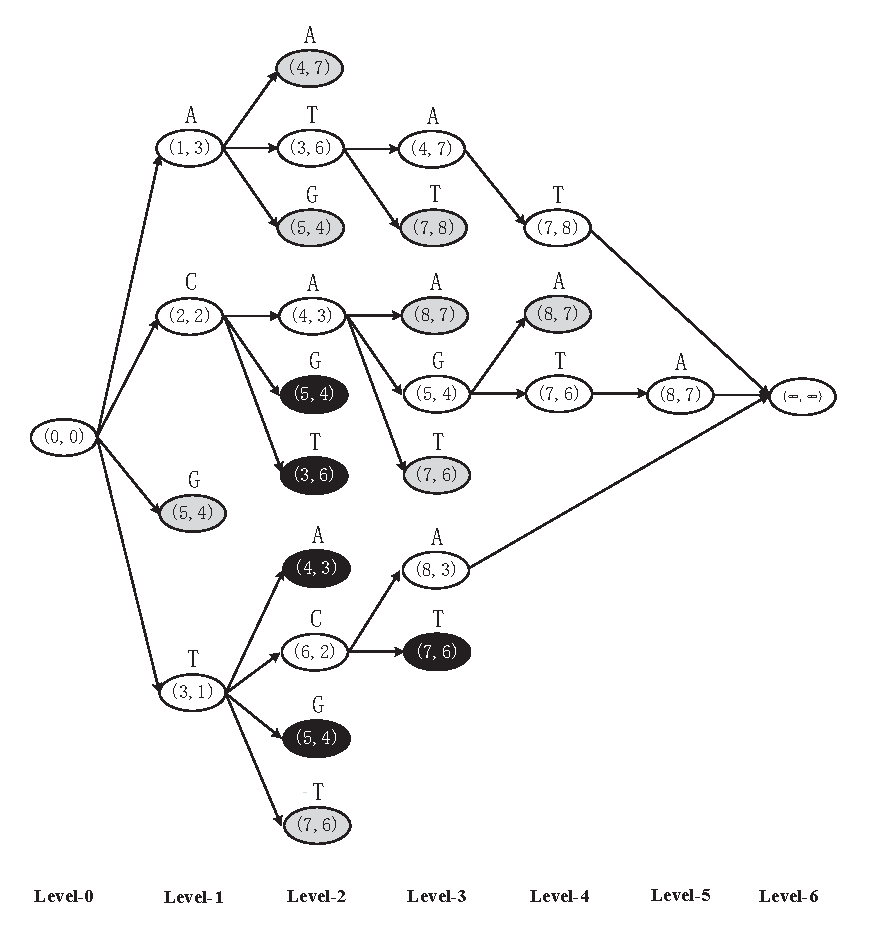
\includegraphics[height=4.5in, width=4.5in]{figures/4_MLCS/DAG}
  \vspace{1.5em}
  \caption{基于支配点模型所构造的有向无环图。图中黑色和灰色的节点将
    被 $Minima$ 剪枝操作删除。}
  \label{fig:DAG}
\end{figure}


\begin{itemize}
\item \textbf{步骤 0}. 产生源节点 $(0,0)$ 和终止节点 $(\infty, \infty)$。
\item \textbf{步骤 1.} 构造图的第一层节点。 对于字符 $A$, 其匹配点 $(1,3)$ 中的两
  个分量分别是 $A$ 在两个输入序列中第一次出现的位置。 这样, 节点 $A(1,3)$ 便是源
  节点在第一层中对应于字符 $A$ 的后继。 类似地, 节点 $C(2,2)$,
  $G(5,4)$ 和 $T(3,1)$ 是源节点分别对应于字符 $C$, $G$ 和 $T$ 的后继。 在第一层的
  这4个节点当中, 通过 \emph{Minima} 剪枝操作找出并删除被支配
  点 $G(5,4)$, 如图 \ref{fig:DAG} 中灰色节点所示。 剩下的3个支配节点构成了图的第
  一层 $D^1=\{A(1,3),C(2,2),T(3,1)\}$。
  
\item \textbf{步骤 2}. 构造图的第二层节点。 对于 $D^1$ 中的每一个节点,
  比如 $A(1,3)$, 由于匹配点 $(4,7)$ 的分量是继匹配点 $(1,3)$ 之后字
  符 $A$ 在两个序列中第一次出现的位置。 这样, 节点 $A(4,7)$ 便是节
  点 $A(1, 3)$ 在第二层中对应于字符 $A$ 的后继。 类似地, 节点 $T(3,6)$
  和 $G(5,4)$ 是节点 $A(1, 3)$ 在第二层中分别对应于字符 $T$ 和 $G$ 的后
  继。 以此类推, 第一层中的节点 $C(2,2)$ 可以产生3个第二层中的后继节点:
  $A(4,3)$, $G(5,3)$ 和 $T(3,6)$,第一层中的节点 $T(3,1)$ 可以产生4个第
  二层中的后继节点: $A(4,3)$, $C(6,2)$, $G(5,4)$ 和 $T(7,6)$。 注
  意, 有些节点会重复产生。 在新产生的第二层的10个节点中, 通过剪枝操
  作 \emph{Minima} 找到并删除重复节点 $A(4,3)$, $G(5,4)$ (会被删除两
  次) 和 $T(3,6)$, 如图第二层中的黑色节点所
  示。 同样, 通过 \emph{Minima} 操作找到并删除被支配节点 $(4, 7)$,
  $(5, 4)$ 和 $(7, 6)$ 如图第二层中的灰色节点所示。 剩余的支配点构成了
  图的第二层 $D^2=\{T(3, 6),\; A(4, 3),\;$ $C(6,2)\}$。 注意, 如果一个
  节点没有任何后继,那么令终止节点为其唯一后继。
\item \textbf{步骤 3}. 逐层重复以上步骤,直到有向无环图构造完毕,即图中所有节
  点(除了终止节点)均已被扩展。
  
\end{itemize}

从以上例子可以看出,基于支配点模型的方法有以下两个缺陷:(1) 每层中会产
生大量重复的,被支配的冗余节点,它们将消耗大量的存储空间。 (2) 找出并删
除冗余节点的剪枝操作需要对大量的 $d$ 维向量进行逐对比较,每次比较又需
要 $d$ 次整数比较,当 $d$ 较大时,对每一层进行剪枝操作将会变得极其耗
时。

Hunt \cite{Hunt1977} 首次提出了针对两个序列的基于支配点的算法,其时间复
杂度为 $O((r+n)logn)$, 其中 $r$ 是支配点图中节点的数量, $n$ 是两个目标
序列的长度。 此后,为了进一步提高算法效率, 各种基于支配点模型的变体算法
被相继提出。Korkin \cite{Korkin2001} 首次提出了并行MLCS求解算法,其时间
复杂度为 $O(|\Sigma||D|)$, 其中 $|D|$ 是支配点图中的节点数量。 Chen
\cite{Chen2006} 提出了一种针对DNA序列的高效算法 -- FAST-LCS, 它采用了一
种被称为后继表的新型数据结构,用来在常量时间内产生一个节点的所有后继,
同时使用了剪枝操作用来删除每一层中的非支配节点。 Wang \cite{Wang2011}
提出了 Quick-DPAR 算法用以改进 FAST-MLCS 算法, 它使用了“分而治之”的策
略来删除非支配点从而使其非常易于并行化, 作者称相比于串行版本的算法,其
并行化算法获得了近似于线性的加速比。Li \cite{Li2012} 和 Yang
\cite{Yang2010} 分别设计了在GPU上针对LCS问题的并行算法和在云平台上针
对MLCS问题的并行化算法。 遗憾的是, 由于过大的同步开销,Yang
\cite{Yang2010} 所提所提算法并不适用于包含很多序列的MLCS问题。 最近,
Li \cite{Li2016_ICDE} 和 Li \cite{Li2016_SIGKDD} 分别提出了两种基于支配
点模型的算法: PTop-MLCS 和 RLP-MLCS, 它们都使用了被称为“无冗余公共子序
列图”(简称为NCSG)的新的图模型, 该图模型在构建过程中能够极大地减少冗余
节点的产生, 同时算法采用了正反向拓扑排序来寻找图中的最长路径。作者称两
种算法的时空复杂度均线性于图中所包含的节点数量。

在实际当中,对于大序列集,传统算法需要花费大量的时间和空间来求解其最优
解(即完整的最长公共子序列集),为解决此问题,一系列近似算法被相继提出。
近似算法首先能够在极短的时间内找出一些次优解 (即非最长公共子序列),然后
通过反复迭代,逐步提高解的质量,最终使其逼近于真实的最优解。Yang
\cite{Yang2013} 提出了基于支配点模型的近似算法--Pro-MLCS及其并行化版
本。 Pro-MLCS 能够以仅仅 $3\%$ 的总运行时间找到近似解, 然后通过反复迭代
来提高解的质量, 迭代时间越长, 解的质量就越好。最近, Yang
\cite{Yang2014} 提出了另外两种近似算法 SA-MLCS 和 SLA-MLCS。 SA-MLCS 使
用了一种称为 “iterative beam widening” 的搜索策略来减少迭代过程中的空
间消耗。 基于 SA-MLCS, 空间受限型算法 SLA-MLCS 被提出, 它可以确保算法运
行时的内存开销不超过预先设定的值。


\section{一种新的图模型---Leveled-DAG 及其构建算法}
\label{sec:Algorithm}

本节中将介绍Leveled-DAG图模型及其相应的构建算法,在描述细节之前,首先介绍一些将要
用到的核心数据结构。

\subsection{核心数据结构}
\label{sec:data structures}

(1). 后继表

高效地产生每一个节点的后继,是构建Leveled-DAG的关键步骤。为此,需要为每
一个输入序列构造一个后继表 \cite{Chen2006}, 通过查询这些后继表,能够在
常量时间内产生一个节点的后继。 具体地,给定序列 $s=c_1c_2...c_n$, 其所
对应的后继表(由 $ST$ 表示)是一个拥有 $|\Sigma| \times (n+1)$ 个元素的二
维数组, 其中第 $i$ 行第 $j$ 列的元素(由$ST[i, j]$表示)按照如下方式计算:

$$ST[i,j]=min\{m\;|\;c_m=\sigma_i,\; m > j,\; 1 \leq i \leq
|\Sigma|,\; 0 \leq j \leq n\}$$

其中 $\sigma_i$ 是字符集 $\Sigma$ 中第 $i$ 个字符。 事实上, $ST[i,j]$
记录了在序列 $s$ 的第 $(j+1)$ 个位置之后,字符 $\sigma_i$ 第一次出现的
位置。 例如, DNA序列 $ACTAGCTA$ 和 $TCAGGTAT$ 的后继表分别在
图 \ref{fig:ST} (a) 和 (b) 中所示。 给定 $d$ 个长为 $n$ 的序列, 其后继
表可以在 $O(d|\Sigma|n)$ 时间内构建完成。

\begin{figure}[!h]
  \centering
  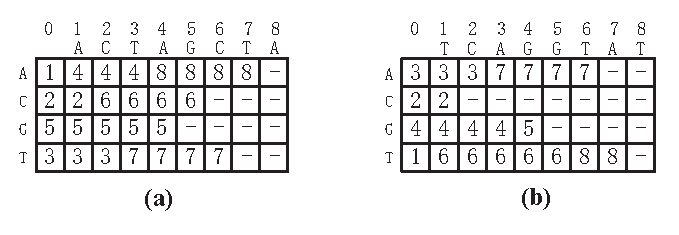
\includegraphics[height=1.2in, width=4.8in]{figures/4_MLCS/successor_table}
  \caption{后继表示例。(a) 序列 ACTAGCTA 的后继表。 (b) 序列 TCAGGTAT
    的后继表。}
    \label{fig:ST}
  \end{figure}

  给定 $d$ 个序列, 通过查询后继表,一个节点的所有后继可以
  在 $O(|\Sigma|d)$ 时间内产生。 例如, 图 \ref{fig:DAG} 中节点 $C(2,
  2)$ 的后继可以通过查讯图\ref{fig:ST}中所示的后继表而得到:
  $(ST_1[1, 2],\;ST_2[1, 2]) = (4, 3)$,\,
  $(ST_1[2, 2],\;ST_2[2, 2]) = (6, -)$,\,
  $(ST_1[3, 2],\;ST_2[3, 2]) = (5, 4)$ and
  $(ST_1[4, 2],\;ST_2[4, 2]) = (3, 6)$, 分别对应于字符 $A$, $C$,
  $G$ 和$T$, 其中 $(6, -)$ 意味着 $(2, 2)$ 没有对应字符 $C$ 的后
  继。 事实上, 一个节点可以没有任何后继。\\

(2). 节点结构
\label{sec:Node}

Leveled-DAG中的每个节点,比如 $t$, 包含了以下信息:

\begin{itemize}
\item 节点 $t$ 所对应的匹配点, 用来标识 $t$ 的唯一性。
\item $Suc(t)$: $t$ 所有后继的集合。
\item $P\_LCS(t)$: 从源节点到 $t$ 的所有最长路径所对应的序列集 (它们是最长公共子
  序列的前缀, 在下文中简称为“前缀序列”)。
\end{itemize}

节点 $t$ 的匹配点用于判断 $t$ 是否已经存在于图中。 后面将会看到, 当一个节点被删除
时,其所包含的前缀序列会由其后继节点继承并加以延长。 当Leveled-DAG构造完毕时,其
中仅剩的终止节点所包含的前缀序列就是要寻找的输入序列的最长公共子序列。\\

(3). 全局数据结构
\label{sec:auxiliary}

\begin{itemize}
\item \emph{L\_DAG} : 用于保存图中的节点。
\item $Cur\_Level$ : 用于保存当前待扩展节点的队列。
\item $Next\_Level$ : 用于保存新产生节点的队列。
\end{itemize}



$L\_DAG$ 是一个映射表结构用于保存图中的节点, 一个节点可以通过其键值(即
匹配点)进行检索。每当一个新节点产生后,通过在 $L\_DAG$ 中检索其匹配点,
可以判断该节点是否已经存在于图中,如果不存在,便将其插
入$L\_DAG$。 队列 $Cur\_Level$ 用于保存当前层中待扩展节点, 而队
列 $Next\_Level$ 用于保存新产生的下一层节点(即当前层中节点的后继)。


\subsection{Leveled-DAG模型}
\label{sec:leveled DAG}

Leveled-DAG模型的核心特性在于,它采用了一种被称为“产生-删除”的策略来
控制图的规模。 具体来说,每当新的一层节点产生之后,图中所有入度为零的节
点(即没有任何边指向其的节点)就会变得“过时”,因为它们不会再是后续产生
节点的后继,其所包含的前缀序列也因此不会再发生变化,所以可以安全地将其
删除而不会对最终结果造成任何影响。通过及时地删除过时节点可以极大地缩小
图的规模并降低内存开销。 基于这种策略,Leveled-DAG将会从源节点开始进行
逐层构造,任意时刻,只有当前新产生层的节点以及(以前产生的)入度不为零的
节点会被保留下来。 一旦构建完成,唯一剩余的终止节点便已包含了所有输入序
列的最长公共子序列,无需任何图搜索操作,这将节省大量运行时间。 下面将给
出一个例子来说明Leveled-DAG模型的构造过程。

\begin{figure}[!h]
  \centering
  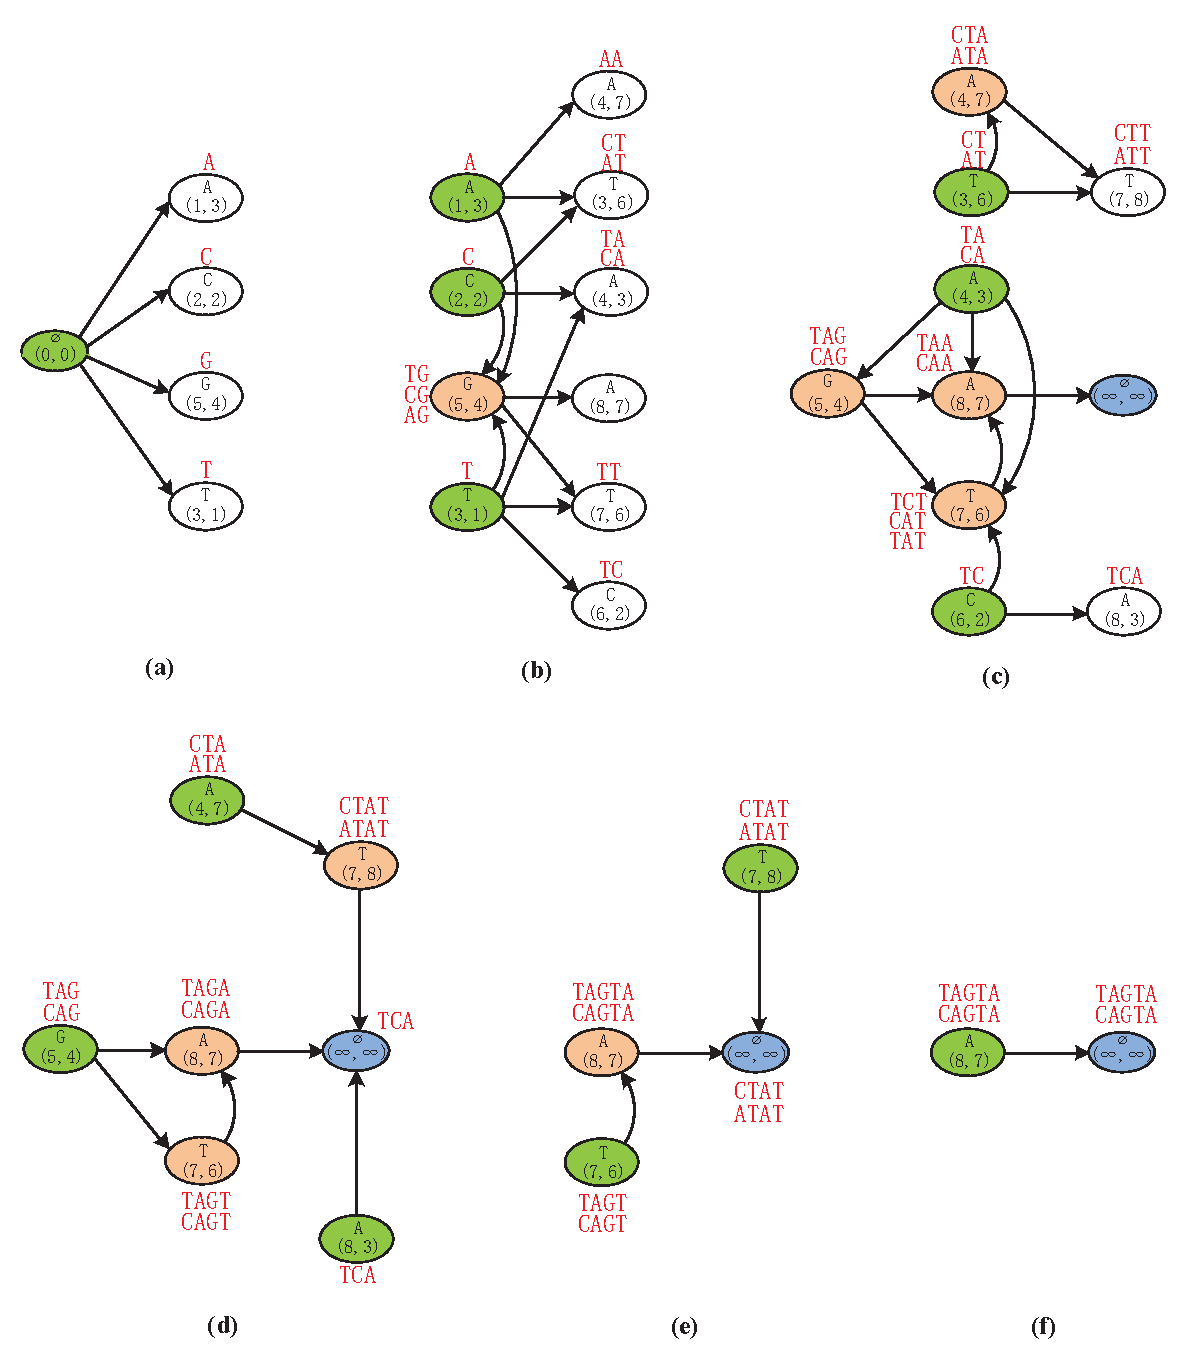
\includegraphics[height=5in,
  width=5in]{figures/4_MLCS/Leveled_DAG}
  \vspace{1.5em}
  \caption{序列 ACTAGCTA 和 TCAGGTAT 所对应的 Leveled-DAG。 匹配点及其
    对应字符在节点内部显示。 节点所对应的前缀序列,由其附近的红色字符串
    表示。 图中白色的节点是新产生的,且稍后将会被扩展。 绿色的节点已经
    过时,即将被删除。 之前产生的带有入边的红色节点,应当予以保留。}
  \label{fig:Leveled-DAG}
\end{figure}

\textbf{例 2.} 基于Leveled-DAG模型求解序列 $ACTAGCTA$ 和 $TCAGGTAT$ 的
最长公共子序列。 最初, Leveled-DAG只包含属于第0层的源节点 $(0, 0)$。 然
后,通过查询图\ref{fig:ST}中所示的后继表,产生源节点的4个后继: $A(1,
3)$, $C(2, 2)$, $G(5, 4)$和 $T(3, 1)$。 由于这4个后继属于第1层,它们的
前缀序列分别是单个字符:$A$, $C$,
$G$ 和 $T$, 如图\ref{fig:Leveled-DAG} (a) 中对应节点上方的红色字符所
示。 此时,由于源节点入度为0,它已经过时,可以从图中安全删除。

然后,产生第1层节点的后继以构成第2层节点,这些后继是: $A(4, 7)$, $T(3,
6)$, $A(4, 3)$, $A(8, 7)$, $T(7, 6)$ 和 $C(6,
2)$, 如图 \ref{fig:Leveled-DAG} (b) 所示。 注意,如果一个后继已经存在
于Leveled-DAG中 (比如 $G(5, 4)$), 它无需再重复产生。 当第2层节点被产生
之后, 由于节点 $A(1, 3)$, $C(2, 2)$ 和 $T(3, 1)$ 入度为0,它们已经过时并
将被删除, 此时, 其所包含的前缀序列需要被其后继节点继承并延长。 例如, 已
经过时的节点 $A(1, 3)$ 有3个后继: $A(4, 7)$, $T(3, 6)$ 和 $G(5, 4)$ (它
没有对应于字符 $C$ 的后继)。 每一个后继都需要将其所对应的字符附加
到 $A(1, 3)$的前缀序列(即 $A$)之后, 然后将延长后的前缀序列作为其自己的
前缀序列。 具体地,后继 $A(4, 7)$ 将 $A$ 附加到 $A$ 之后, 然后将 $AA$作
为自己的前缀序列。 后继 $T(3, 6)$ 将 $T$ 附加到 $A$ 之后, 然后将 $AT$
作为自己的前缀序列。 类似地,后继 $G(5, 4)$ 将 $G$ 附加
到 $A$之后, 将 $AG$ 作为自己的前缀序列。 注意, 由于 $G(5, 4)$ 同时是
这3个过时节点的后继, 它通过继承并延长这3个节点的前缀序列, 得到了自己
的3个前缀序列,分别是: $TG$, $CG$ 和 $AG$。 在移除过时节点之后,图中仅
剩余7个节点。

接下来, 如图 \ref{fig:Leveled-DAG} (c) 所示, 产生第2层所有节点的所有后
继:$T(7, 8)$ 和 $A(8, 3)$ 构成图的第3层。 注意, 由于节点 $A(8, 7)$ 没
有任何后继, 令终止节点 $(\infty, \infty)$ 为其唯一后继。 在第3层构建完
毕之后, 节点 $T(3, 6)$, $A(4, 3)$ 和 $C(6, 2)$ 已经过时。 在移除它们之
前, 其所包含的前缀序列需要被其后继节点继承并延长。 作为特
例, 由于 $A(4, 7)$ 是过时节点 $T(3, 6)$ 的一个后继, $T(3, 6)$ 的前缀序
列 $CT$ 和 $AT$, 将由 $A(4, 7)$ 继承并加以延长(附加 $A$)。 由于延长后
的前缀序列 $CTA$ 和 $ATA$ 比 $A(4, 7)$ 原有的前缀序列 $AA$ 要
长, $A(4, 7)$ 的前缀序列将被相应地更新为 $CTA$ 和 $ATA$。 类似
地, 节点 $G(5, 4)$ 和 $T(7, 6)$ 的前缀序列同样通过继承并延长其过时前驱
的前缀序列加以更新。

如图 \ref{fig:Leveled-DAG} (d) 所示, 需要扩展新产生的第3层中的节
点 $T(7, 8)$ 和 $A(8, 3)$。 由于这两个节点均没有后继, 终止节点将被定义
为这两个节点的唯一后继。 由于没有新的节点产生, 此后将不再需要扩展任何节
点。 从此刻起,算法只需要不断地删除过时节点,并更新其相应后继节点的前缀
序列。 当前, 节点 $A(4, 7)$, $G(5, 4)$ 和 $A(8, 3)$ 将被移除。 通过继
承 $A(8, 3)$ 的前缀序列 $TCA$, 终止节点将其作为自身的前缀序列 (终止节
点不附加任何字符)。 接着, 如图 \ref{fig:Leveled-DAG}
(e) 所示, 节点 $T(7, 6)$ 和 $T(7, 8)$ 将被移除, 相应地,终止节点的前缀
序列将被更新为 $CTAT$ 和 $ATAT$。 最终, 如图 \ref{fig:Leveled-DAG} (f)
所示, 在移除最后一个过时节点 $A(8, 7)$ 之后, 终止节点的前缀序列会被更新
为 $TAGTA$ 和 $CAGTA$, 它们即是输入序列的最长公共子序列。

从以上例子可以看到, 最初仅有一个源节点存在于Leveled-DAG中, 然后节点的数量将不断增
加, 一旦不再有新的节点产生, 节点的数量将开始下降直到剩余终止节点。 在此过程中, 只
有新产生的节点和以前产生的入度不为0的节点会被保留在Leveled-DAG中, 极大地减少了存
储开销。 当Leveled-DAG构建结束后, 输入序列的最长公共子序列立即可得。

\subsection{Leveled-DAG 模型的构建算法 }
\label{sec:PMA}

本节将给出Leveled-DAG模型构建算法的形式化描述。\\

\textbf{算法 1.} 构建 Leveled-DAG
\begin{itemize}
\item \textbf{步骤 0.} 预处理。 对每一个输入序列,构造其后继表。
\item \textbf{步骤 1.} 构建Leveled-DAG的第一层。通过查询后继表产生源节点的所有后
  继,作为图的第一层。 令每一个后继所对应的字符作为其(单字符)前缀序列。删除源节
  点。
\item \textbf{步骤 2.} 产生Leveled-DAG的下一层节点并删除过时节
  点 (即“产生-删除”策略)。 如果在Leveled-DAG中存在未扩展节点, 则重复以下两个子
  步骤:
  \begin{itemize}
  \item \textbf{步骤 2.1(产生).} 对每一个未扩展节点 $t$, 产生 $t$ 的所有后继 (如果某个
    后继已经存在于图中,无需重复产生, 只需通过指针建立其与 $t$ 的后继关系)。 如
    果 $t$ 没有后继,令终止节点作为其唯一后继。
  \item \textbf{步骤 2.2 (删除).} 令 $|p|$ 表示节点 $p$ 所包含前缀序列
    的长度。 对每一个入度为0的节点 $p$, 以及 $p$ 的每一个后继 $s$, 执行:
    \begin{itemize}
    \item 如果 $|p| \geq |s|$, 则删除 $s$ 原有的前缀序列。 将 $s$ 所对
      应的字符附加到 $p$ 的每一个前缀序列之后, 将这些延长后的前缀序列
      作为 $s$ 的(新的)前缀序列加以保存。
    \item 否则,如果 $|p| = |s|-1$, 则将 $s$ 所对应的字符附加到 $p$ 的
      每一个前缀序列之后, 并将这些延长后的前缀序列添加到 $s$ 原有的前
      缀序列集中。
    \end{itemize}
    删除节点 $p$ 及其前缀序列集。
  \end{itemize}
\item \textbf{步骤 3.} 重复执行步骤 2.2, 直到剩余终止节点。
\item \textbf{步骤 4.} 输出终止节点所保存的前缀序列,即输入序列的最长公共子序列。
\end{itemize}

如算法 1中所示, 在预处理 (步骤 0) 之后, Leveled-DAG最初只包含源节点(步
骤 1), 然后它采用“产生-删除”策略来产生下一层节点 (步骤 2.1) 和删除过
时节点 (步骤 2.2), 一旦Leveled-DAG中所有的节点都被扩展, 即不再有新节点
产生, 算法开始重复地删除过时节点 (步骤 3), 直到剩余终止节点。 最后,输出
终止节点所保存的前缀序列,即输入序列的最长公共子序列(步骤 4)。

下面给出了算法1的伪代码描述, 其中所用到的数据结构在 \ref{sec:data
  structures} 节已经介绍, 构造后继表的过程已经省略, 后继表被直接作为输
入数据。 算法1中的步骤1和步骤2被合并为一个 \emph{while} 循环 (7 $\sim$
22行), 步骤3对应于随后的 \emph{while} 循环 (24 $\sim$ 26行)。 移除过时
节点的操作被封装为一个独立函数 $Remove\_Outdated$, 对应于 30 $\sim$
49行。

\begin{algorithm}
  \caption{伪代码}
  \footnotesize
  \label{alg:PMA}
  \begin{algorithmic}[1]
    \REQUIRE ~~\\
    输入序列的后继表。\\
    \ENSURE ~~\\
    输入序列的最长公共子序列。
    \STATE
    \STATE $Suc(source) \leftarrow \emptyset$, $P\_LCS(source) \leftarrow \emptyset$
    \STATE $Suc(end) \leftarrow \emptyset$, $P\_LCS(end) \leftarrow \emptyset$
    \STATE $L\_DAG \leftarrow \{source, end\}$
    \STATE $Cur\_Level \leftarrow \{source\}$
    \STATE
    \WHILE{$Cur\_Level \neq \emptyset$}
    \FOR {每一个节点 $t \in Cur\_Level$}
    \FOR {$t$ 的每一个后继 $s$}
    \STATE $Suc(t) \leftarrow Suc(t) \cup \{s\}$
    \IF{$s \notin L\_DAG$}
    \STATE $L\_DAG \leftarrow L\_DAG \cup \{s\}$
    \STATE $Next\_Level \leftarrow Next\_Level \cup \{s\}$
    \ENDIF
    \ENDFOR
    \IF{$t$ 没有后继}
    \STATE $Suc(t) \leftarrow \{end\}$
    \ENDIF
    \ENDFOR
    \STATE $Remove\_Outdated(L\_DAG)$
    \STATE $Cur\_Level \leftarrow Next\_Level$
    \ENDWHILE
    \STATE
    \WHILE {$\exists t \in L\_DAG$ and $t \neq end$}
    \STATE $Remove\_Outdated(L\_DAG)$
    \ENDWHILE
    \STATE
    \STATE 输出: $P\_LCS(end)$
    \STATE
    \STATE $Remove\_Outdated(L\_DAG):$
    \FOR {每一个入度为零的节点 $p \in L\_DAG$}
    \FOR {$p$ 的每一个后继 $s$}
    \STATE $|p| \leftarrow $ $p$ 所包含前缀序列的长度
    \STATE $|s| \leftarrow $ $s$ 所包含前缀序列的长度
    \STATE $\delta \leftarrow $ 节点 $s$ 所对应的字符
    \IF {$|p| \geq |s|$}
    \FOR {每一个 $plcs \in P\_LCS(p)$}
    \STATE 将 $\delta$ 附加到 $plcs$ 末尾
    \ENDFOR
    \STATE $P\_LCS(s) \leftarrow $ \{所有延长后的前缀序列\} 
    \ELSIF {$|p| + 1 = |s|$}
    \FOR {每一个 $plcs \in P\_LCS(p)$}
    \STATE 将 $\delta$ 附加到 $plcs$ 末尾
    \ENDFOR
    \STATE $P\_LCS(s) \leftarrow P\_LCS(s) \cup \{$所有延长后的前缀序列$\}$
    \ENDIF
    \STATE 从 $L\_DAG$ 中删除 $p$
    \ENDFOR
    \ENDFOR
  \end{algorithmic}
\end{algorithm}

\subsection{时间/空间复杂度分析}
\label{sec:complexity}

接下来将给出Leveled-DAG方法粗略的时间/空间复杂度估计。如上所述,
Leveled-DAG方法包含两个阶段: 1. 为每一个输入序列构造后继表; 2.基于后继
表构造Leveled-DAG图。 第一个阶段, 如 \ref{sec:data structures} 节所
示,对长为$n$ 的序列,构造其后继表将花费 $O(|\Sigma|n)$ 时间, 因此,
为 $d$个长为 $n$ 的序列构造后继表将花费 $O(d|\Sigma|n)$ 时间。 对于第二
个阶段, 从宏观角度来看, 构造Leveled-DAG 图的过程仅仅是产生出所有图节点
然后再将其全部删除 (除了终止节点)。 尽管产生节点和删除节点在构建过程中
交织在一起, 图中任意节点仅被产生并删除一次, 并且整个构建过程不含任何递
归调用 (见算法1的伪代码描述)。 因此, 构建图的时间复杂度
为$O(2|Nodes|)$, 其中 $|Nodes|$ 为产生的节点数量, 产生节点和删除节点的
过程都需要$O(|Nodes|)$ 时间。 结合这两个阶段, Leveled-DAG方法的时间复杂
度为 $O(d|\Sigma|n + 2|Nodes|)$。 由于总是有 $O(d|\Sigma|n) \ll
O(2|Nodes|)$
(由实验证实),所以$O(d|\Sigma|n + 2|Nodes|) = O(2|Nodes|) =
O(|Nodes|)$, 这意味着Leveled-DAG方法的时间复杂度与图中节点的数量呈线性
关系。

对于空间复杂度, 一方面, Leveled-DAG 方法需要存储所有的后继表,这需
要 $O(d|\Sigma|(n+1))$ 的存储空间。 另一方面, 如前所述, Leveled-DAG 图主要需要保
存最新产生的一层节点, 且最新一层节点的数量会先增后降, 因此Leveled-DAG方法的内存开
销也会先增后降。 所以, Leveled-DAG方法的峰值内存消耗
为 $O(|Max\_Level|)$, 其中 $|Max\_Level|$ 是图中最大一层所包含节点的数量。 结合两
方面内存开销, Leveled-DAG方法的空间复杂度为 $O(d|\Sigma|(n+1) + |Max\_Level|)$,
由于总是有 $O(d|\Sigma|(n+1)) \ll O(|Max\_Level|)$, 所以
$O(d|\Sigma|(n+1) + |Max\_Level|) = O(|Max\_Level|)$, 这意味
着Leveled-DAG方法的空间复杂度主要取决于图中最大一层的节点数量。


\section{实验结果}
\label{sec:4_experiments}

本节将使用真实的生物序列,从时间和空间两方面来比较Leveled-DAG方法和其它三个主
流MLCS算法: \emph{Top\_MLCS} \cite{Li2016_ICDE}, \emph{Quick-DP}
\cite{Wang2011} 和 \emph{Fast\_LCS} \cite{Chen2006} 的性能。

\subsection{实验设定}
\label{Test problems}

实验将使用两种类型的生物序列: DNA序列 ($|\Sigma|=4$) 和蛋白质序
列 ($|\Sigma|=20$) 作为输入数据。 我们将进行两方面的实验:

\begin{enumerate}
\item 测试不同数量的序列: 对每一种类型的生物序列, 序列的长度固定为100,数量由3逐
  步增加到700。
\item 测试不同长度的序列: 对每一种类型的生物序列, 序列的数量固定为5个,长度由50逐
  步增加到5000。
\end{enumerate}

对每次实验, 根据指定的长度和数量,输入序列由一个大的原始序列集中随机抽取而产
生。 所有测试算法均由C/C++实现,由gcc编译器编译(-O2), 在同一台服务器上运行,配置
为: Intel Xeon E7-8880 2.2 GHz CPU, 700 GB内存 (由于服务器被多个用户共享,分配给
每个进程的内存被限定为300GB)。操作系统为 GNU/Linux (amd64)。

\subsection{测试不同数量的序列}
\label{sec:number}

在第一种实验中,所有输入序列的长度均被固定为100, 序列的数量由3逐渐增加到700。 将
对DNA和蛋白质两种序列分别进行实验。 所有算法独立运行5次,使用32个线程,它们的平
均CPU占用时间(以及运行时间的标准差)和内存消耗被测量并分别显示于
表 \ref{tab:times1} 和表 \ref{tab:memory1} 中。 值得指出的是, 算法的运行时间和内
存消耗高度依赖于序列本身, 即使两个序列集包含相同数量和长度的序列, 如果其包含序列
本身不同, 算法在这两个序列集上的运行时间和内存消耗可能变化很大。

实验结果显示, 由于内存溢出,\emph{FAST\_LCS} 和 \emph{Quick-DP} 算法无法处理包
含20个或更多序列的序列集。 如表 \ref{tab:memory1} 所示, 这两个算法的内存占用相当
接近 (因为它们采用了同样的框架,唯一不同之处在于删除非支配节点的方式), 并且都随着
序列数量的增加呈指数增长, 这是因为二者都需要产生大量的冗余节点,并将其保存在内存
中。 如表 \ref{tab:times1} 所示, 它们的运行时间也随着序列数量的增长而快速增长,这
是因为随着序列个数的增加,每个节点所包含的匹配点的维数也相应增加。 因此, 为了删除
非支配节点, 两个算法所使用的 \emph{Minima} 操作需要在每一层中对所有节点的匹配向量
进行逐维度比较。 这需要大量的比较操作且非常耗时。 另一方面, \emph{Quick-DP} 相比
较 \emph{FAST\_LCS} 要快很多,因为它采用了非常适于并行化的分而治之的策略来删除非
支配点。 遗憾的是, \emph{Quick-DP} 算法在应对包含很多序列的序列集时,无论在时间或
空间方面仍然不够高效。

作为对比, 从试验结果可以看出 \emph{Top\_MLCS} 算法和本章提出
的 \emph{Leveled-DAG} 算法都可以处理高达 700 个序
列。 如表 \ref{tab:memory1} 所示, 二者的内存占用相比前两个算法都大幅减少, 这是因为
它们都采用了新的图模型来减小支配点图的规模: \emph{Top\_MLCS} 算法所用
的 \emph{ICSG} 模型不会产生冗余节点, 而 \emph{Leveled-DAG} 模型仅需要保存当前层及
以前层的一部分节点。 相比 \emph{Top\_MLCS}, \emph{Leveled-DAG} 算法对于(数量超
过100的)DNA和蛋白质序列,分别能够节省大约 $35\% \sim 40\%$ $/$ $33\% \sim 35\%$
的存储空间, 这是由于对于规模较大的序列集,Leveled-DAG所保存的(最大)节点数量(包括
最大一层的节点和以前层的入度非0的节点) 大约只占节点总数的 $40\%$。 需要注意的是,
起初两个算法的内存开销都会随着序列数量的增加而快速增长, 但是当序列数量增加到某个
特定值时 (本实验中,大约在 $80 \sim 90$ 之间), 算法的内存增长率开始降低, 且最终
算法的内存增长趋向常量。 我们发现,这是由于当序列的数量增长到某个特定的临界值时,
节点数量的增长率开始下降 (临界值非常难以确定,因为它由许多因素决定,比如序列的字
符集, 序列的长度和序列本身), 并且随着序列数量的进一步增长,图中的节点数量将保持大
致不变, 此时的空间增长主要来自于每个节点内部匹配点维数的增加。

时间方面, 两个算法比都比 \emph{FAST\_LCS} 和 \emph{Quick-DP} 算法快一到两个数量
级,(且其运行时间的增长率,随着序列的增加将会下降)。 这主要是由于二者不需要类似
于 \emph{FAST\_LCS} 和 \emph{Quick-DP} 算法所使用的 \emph{Minima} 操作来对匹配点
进行逐对比较。 相比 \emph{Top\_MLCS} 算法, \emph{Leveled-DAG} 对于较小的序列集
(包含少于10个序列) 大约快 $10\%$, 对于更大的序列集,大约快 $10\%$ $\sim$
$20\%$。 这是因为 \emph{Top\_MLCS} 算法在支配点图构造好之后,还需要进行两趟拓扑排
序 (正向和反向拓扑排序) 才能找到目标序列的最长公共子序列,而 \emph{Leveled-DAG}
算法在建图完成之后无需任何搜索操作。 事实上, 所需的最长公共子序列已经保存在终止节
点中了, 立即可得。 总上所述, \emph{Leveled-DAG} 算法相比其它算法更加适用于处理大
序列集。

从表 \ref{tab:times1} 和表 \ref{tab:memory1} 可以看出, 对于蛋白质序列,所有测试算
法的效率(在时间和空间两方面)都优于DNA序列, 这是由于对于大字符集序列(比如蛋白
质) 其所对应的支配点图要小于相应的小字符集序列(比如DNA)的支配点图。稍后将对此进行
深入讨论。


\subsection{测试不同长度的序列}
\label{sec:times2}

在第二种类型的实验中, 序列数量固定为5, 序列长度由 50 逐步增加到 5000。 同上, 所有
算法使用32个线程独立运行5次, 它们的平均运行时间 (及运行时间的标准差) 和内存消耗分
别在表 \ref{tab:times2} 和 表 \ref{tab:memory2} 中列出。

从实验结果可得, 由于运行时间过长, \emph{FAST\_LCS} 算法无法处理长度超
过400的DNA序列和长度超过500的蛋白质序列; 由于内存溢出, \emph{Quick-DP} 算法无法
处理长度超过800的DNA序列和长度超过1000的蛋白质序列。 (算法处理蛋白质序列的性能要
优于处理DNA序列的性能)。 这是因为随着序列长度的增加,算法所构建的图的层数也会相应
地增加, 这样每层所包含的节点数量将会呈指数增长, 使得所构建的图占用过多的存储空
间。 同样, \emph{FAST\_LCS} 和 \emph{Quick-DP} 算法的运行时间也随着序列长度的增加
而快速增加, 主要原因是每层的节点数量将会随着层数的增加而呈指数级增长,使得在每层
上执行 \emph{Minima} 剪枝操作变得极其耗时, 另外,在包含很多层的图中搜索最长公共子
序列会花费更多的时间。 因此, 这两种算法都不适用于寻找长序列的最长公共子序列。

另一方面, 如表 \ref{tab:memory2} 所示, \emph{Top\_MLCS} 算法
和 \emph{Leveled-DAG} 算法可以处理长度为5000的DNA序列或蛋白质序列。 对于长度超
过1000的DNA/蛋白质序列,相比于 \emph{Top\_MLCS} 算法, \emph{Leveled-DAG} 算法可以
节省大约 $43\% \sim 46\%$ $/$ $41\% \sim 45\%$ 的内存空间, 这是由
于 \emph{Leveled-DAG} 的内存开销主要取决于图中最大层的节点数量, 而最大层节点数在
节点总数中所占比例会随着序列长度的增加而逐渐下降。 时间方面,如
表 \ref{tab:times2} 所示, 这两个算法运行时间的增长相
比 \emph{FAST\_LCS} 和\emph{Quick-DP} 算法要缓慢得多。 即使对于长序列
集 ($长度 \geq 1000$), \emph{Top\_MLCS} 和 \emph{Leveled-DAG} 算法仍然可以有效地
找出其最长公共子序列。 值得注意的是, 在所有情形, 所提的 \emph{Leveled-DAG} 算法
都是最快的: 至少比 \emph{FAST\_LCS} 和 \emph{Quick-DP} 算法快两个数量级; 在长序
列集上($长度 \geq 2000$), 比 \emph{Top\_MLCS} 快大
约 $20\%$ 。 \emph{Leveled-DAG} 算法比 \emph{Top\_MLCS} 快的原因是, 随着序列长度
的增长, \emph{Top\_MLCS} 所用的前向拓扑排序过程将会花费过多的时
间, 而 \emph{Leveled-DAG} 的性能变化受序列长度的影响较小。

综上所述, 由于所构图规模较小以及逐渐生成最长公共子序列的技
术, \emph{Leveled-DAG} 算法在所有测试集上都有更好的表现,尤其对于包含
多个序列或长序列的序列集。

\subsection{进一步分析}

下面将分析影响MLCS算法性能的一些重要因素。序列长度是影响算法性能的关键
因素之一: 对同一类型的序列,随着序列长度增加,算法所构建图中所包含的层
数会相应地增加。 由于每层的节点数会随着层数的增长呈(接近)指数增长, 图中
所包含的节点总数将会随着序列长度的增加而激增。所以,相比短序列集,算法
对于长序列集所建图的规模会更大,相应地, 算法在寻找长序列集的最长公共子
序列的时间和空间开销均大于处理短序列集的开销。 另一方面, 序列的数量也会
对算法性能造成影响: 随着序列数量的增加, 每个节点所包含匹配点的维数也会
相应增加, 因此, 图中每个节点将会占用更多的空间。 而且,比较两个匹配点
也将花费更多的时间。 另外, 序列的数量和长度也会影响算法的最终结果: 很明
显, 序列越长, 所求得的最长公共子序列越长; 相反地, 序列数量越多,所求得
的最长公共子序列越短。

从实验结果可以发现, 序列的字符集可以对算法性能造成很大影响。算法在处理
较大字符集序列 (比如蛋白质)时的性能要优于处理较小字符集序列(比如DNA序
列)时的性能。 这是因为, 对于定长序列, 字符集越大, 每个字符在序列中出现
的次数相对越少,这意味着对于大字符集序列, 算法所建图中的节点与其后继节
点之间的“距离”会变长, 相应地,图中所包含的层数也会变少。 例如, 当序列
长度固定为100时, 算法对DNA序列所构造的图大约有30层,而对蛋白质序列所构造
的图大约只有10层。 尽管对于同一层来说, 蛋白质图中所包含的节点要多
于DNA图中所包含的节点 (因为蛋白质图中每个节点可以拥有多达20个后
继, 而DNA图中的一个节点最多只有4个后继), 蛋白质序列图的节点总数仍然少
于DNA序列图的节点总数。 相应地, 算法对于大字符集序列的性能要优于小字符
集序列的性能。

\section{本章小节}
\label{sec:4_conculsion}

本章提出了一种新的求解MLCS问题的图模型---Leveled-DAG, 它比现有的图模型
在规模上要小很多,同时基于该模型, 给出了相应的构建算
法。 一旦Leveled-DAG构建完成, 所需的最长公共子序列便保存在唯一剩余的终
止节点中,无需任何搜索操作。 实验结果证实,所提方法对所有测试序列集均非
常高效, 尤其对包含很多序列或长序列的序列集。

通过分析程序, 我们发现 Leveled-DAG 方法中最耗时的部分是删除过时节点的操
作 (即算法2中的 $Remove\_Outdated(L\_DAG)$ 函数, 大约占算法总运行时间
的 $50\% \sim 60\%$), 尤其是将某个过时节点的前缀序列传递给其后继的过
程。 该过程需要大量的内存分配、 调整大小、 以及释放操作, 这些操作都不适
宜并行化因此非常耗时。 为了提升性能, 我们将关注于更高效的传递策略及更精
细的编码实现。 我们同样寻求于更高效的内存管理函数来取代当前程序中所用的
由标准库提供的内存分配函数。



\begin{table*}[htp]
  \footnotesize
  \topcaption{对比算法在包含不同数量序列的序列集上的平均运行时间(单位为秒)。 序列长度
    固定为100。 括号中为运行时间的标准差。}
  \label{tab:times1}
\resizebox{6.5in}{!}{
  \begin{tabular}{|r|r|r|r|r|r|r|r|r|r|}
    \hline
    Number &
    \multicolumn{4}{c|}{DNA ($|\Sigma|=4$)} & \multicolumn{4}{c|}{Protein ($|\Sigma|=20$)}\\
    \cline{2-9}
      & FAST\_LCS & Quick-DP & Top\_MLCS & Leveled-DAG & FAST\_LCS & Quick-DP & Top\_MLCS & Leveled-DAG \\
    \hline
    3  & 0.052 (0.003)    & 0.041 (0.001)  & 0.031 (0.002)  & 0.018 (0.001)  & 0.021 (0.001)    & 0.034 (0.002)  & 0.027 (0.001)  & 0.016 (0.001) \\
    4  & 0.255 (0.01)     & 0.203 (0.02)   & 0.071 (0.004)  & 0.053 (0.003)  & 0.183 (0.02)     & 0.152 (0.03)   & 0.051 (0.003)  & 0.037 (0.002) \\
    5  & 2.9 (0.1)        & 1.5 (0.09)     & 0.12 (0.008)   & 0.082 (0.004)  & 2.1 (0.1)        & 1.0 (0.08)     & 0.098 (0.008)  & 0.077 (0.006) \\
    6  & 26.5 (1.7)       & 10.3 (0.8)     & 1.3 (0.09)     & 1.1 (0.1)      & 20.8 (1.2)       & 6.9 (0.6)      & 0.94 (0.03)    & 0.75 (0.02)  \\
    7  & 151.8 (10.0)     & 32.8 (1.9)     & 3.6 (0.1)      & 2.7 (0.2)      & 116.5 (10.3)     & 21.8 (1.3)     & 2.8 (0.2)      & 1.9 (0.1) \\
    8  & 834.9 (43.8)     & 147.6 (8.8)    & 8.5 (0.6)      & 6.9 (0.4)      & 746.5 (58.8)     & 107.0 (8.7)    & 6.3 (0.3)      & 4.7 (0.2) \\
    9  & 4174.6 (408.7)   & 738.5 (51.5)   & 16.4 (0.9)     & 13.7 (0.6)     & 3059.2 (301.4)   & 585.6 (40.2)   & 12.5 (0.8)     & 9.9 (0.4) \\
                                                                                                                                  
    10 & 25671.4 (2433.8) & 3385.4 (326.4) & 30.0 (2.3)     & 25.3 (0.9)     & 22751.9 (1596.7) & 2645.3 (215.7) & 24.7 (1.5)     & 20.6 (1.1)  \\
    20 & --               & --             & 64.8 (4.6)     & 51.2 (2.1)     &  --              &  --            & 57.7 (3.3)     & 45.3 (2.3)  \\
    30 & --               & --             & 136.7 (6.7)    & 96.7 (3.7)     &  --              &  --            & 124.3 (8.9)    & 89.2 (4.7)  \\
    40 & --               & --             & 250.3 (9.4)    & 191.4 (7.5)    &  --              &  --            & 223.4 (14.7)   & 180.8 (10.5) \\
    50 & --               & --             & 463.2 (17.5)   & 380.1 (12.3)   &  --              &  --            & 432.7 (22.4)   & 366.4 (16.0) \\
    60 & --               & --             & 665.4 (42.2)   & 530.3 (27.4)   &  --              &  --            & 590.6 (31.2)   & 509.5 (20.4) \\
    70 & --               & --             & 1088.1 (76.7)  & 875.5 (39.4)   &  --              &  --            & 967.8 (76.4)   & 848.6 (39.6) \\
    80 & --               & --             & 1684.6 (127.5) & 1233.2 (62.3)  &  --              &  --            & 1432.6 (105.2) & 1167.0 (66.8) \\
    90 & --               & --             & 2217.9 (188.3) & 1764.6 (85.5)  &  --              &  --            & 2053.5 (127.1) & 1715.1 (84.1) \\
                                                                                                                                  
    100& --               & --             & 3041.5 (220.9) & 2417.8 (174.9) &  --              &  --            & 2320.2 (144.8) & 2056.2 (101.5)\\
    200& --               & --             & 3398.3 (241.4) & 2778.2 (190.2) &  --              &  --            & 2492.6 (152.4) & 2118.5 (114.9) \\
    300& --               & --             & 3665.0 (263.8) & 2962.5 (206.7) &  --              &  --            & 2614.2 (165.7) & 2214.3 (138.8) \\
    400& --               & --             & 3981.6 (285.0) & 3191.2 (218.0) &  --              &  --            & 2745.3 (172.8) & 2375.4 (152.9) \\
    500& --               & --             & 4237.2 (310.3) & 3384.0 (231.4) &  --              &  --            & 2862.4 (181.1) & 2435.1 (164.3) \\
    600& --               & --             & 4555.9 (336.9) & 3547.2 (243.7) &  --              &  --            & 2947.9 (193.4) & 2479.2 (170.7)\\
    700& --               & --             & 4880.3 (362.7) & 3854.7 (266.2) &  --              &  --            & 3174.8 (204.5) & 2511.9 (183.2)\\
    \hline
  \end{tabular}
  }
\end{table*}

\begin{table*}[htp]
  \footnotesize
  \topcaption{对比算法在包含不同数量序列的序列集上的内存占用量(单位为MB)。序列长度固
    定为100。}
  \label{tab:memory1}
\resizebox{6.5in}{!}{ \begin{tabular}{|r|r|r|r|r|r|r|r|r|r|}
   \hline
   Number &
   \multicolumn{4}{c|}{DNA ($|\Sigma|=4$)} & \multicolumn{4}{c|}{Protein ($|\Sigma|=20$)}\\
   \cline{2-9}
     & FAST\_LCS & Quick-DP & Top\_MLCS & Leveled-DAG & FAST\_LCS & Quick-DP & Top\_MLCS & Leveled-DAG \\
   \hline
   3  & 28      & 31      &  8        & 5      & 25     & 28    & 7      & 4   \\
   4  & 373     & 447     &  23       & 17     & 330    & 403   & 19     & 14  \\
   5  & 1358    & 1485    &  93       & 85     & 1167   & 1304  & 77     & 62  \\
   6  & 3315    & 3490    &  297      & 223    & 2718   & 2960  & 203    & 190 \\
   7  & 5190    & 5862    &  534      & 489    & 4152   & 4706  & 469    & 418 \\
   8  & 11057   & 12051   &  1211     & 1124   & 8513   & 9871  & 1017   & 943 \\
   9  & 20634   & 21183   &  3058     & 2765   & 15138  & 16062 & 2538   & 2238\\

   10 & 35769   & 36934   &  5813     & 5232   & 25637  & 26048 & 4766   & 4251  \\
   20 & --      & --      &  32329    & 28126  &  --    &  --   & 24246  & 18045 \\
   30 & --      & --      &  48765    & 39291  &  --    &  --   & 36824  & 26713  \\
   40 & --      & --      &  67813    & 52607  &  --    &  --   & 49503  & 35182  \\
   50 & --      & --      &  91128    & 68103  &  --    &  --   & 64292  & 46137  \\
   60 & --      & --      &  121268   & 87359  &  --    &  --   & 81379  & 58174  \\
   70 & --      & --      &  156470   & 118600 &  --    &  --   & 98541  & 61036  \\
   80 & --      & --      &  197387   & 141859 &  --    &  --   & 117390 & 76283  \\
   90 & --      & --      &  209145   & 146402 &  --    &  --   & 120833 & 81429  \\


   100& --      & --      &  229372   & 151386 &  --    &  --   & 124124 & 84069  \\
   200& --      & --      &  252247   & 163948 &  --    &  --   & 131920 & 88132  \\
   300& --      & --      &  261963   & 167085 &  --    &  --   & 138255 & 92025  \\
   400& --      & --      &  268993   & 170811 &  --    &  --   & 144213 & 96044  \\
   500& --      & --      &  276103   & 173945 &  --    &  --   & 151318 & 101250 \\
   600& --      & --      &  290398   & 177140 &  --    &  --   & 157986 & 104986 \\
   700& --      & --      &  299498   & 179846 &  --    &  --   & 162298 & 108107 \\
   \hline
  \end{tabular}}
\end{table*}





\begin{table*}[htp]
  \footnotesize
  \topcaption{对比算法在包含不同长度序列的序列集上的平均运行时间(单位为秒)。 序列个数
    固定为5。 括号中为运行时间的标准差。}
  \label{tab:times2}
  \resizebox{6.5in}{!}{
  \begin{tabular}{|r|r|r|r|r|r|r|r|r|r|}
     \hline
    Length &
    \multicolumn{4}{c|}{DNA ($|\Sigma|=4$)} & \multicolumn{4}{c|}{Protein ($|\Sigma|=20$)}\\
    \cline{2-9}
     & FAST\_LCS & Quick-DP & Top\_MLCS & Leveled-DAG & FAST\_LCS & Quick-DP & Top\_MLCS & Leveled-DAG \\
    \hline
    50   & 0.57 (0.03)   & 0.13 (0.01)     & 0.038 (0.002)   & 0.026 (0.001)    & 0.06 (0.001)   & 0.018 (0.001)    & 0.004 (0)     & 0.001 (0) \\
    100  & 2.7 (0.2)     & 1.4 (0.08)      & 0.23 (0.03)     & 0.96 (0.04)      & 0.3 (0.02)     & 0.16 (0.01)      & 0.077 (0.003) & 0.058 (0.006)\\
    200  & 244.1 (10.4)  & 10.6 (0.2)      & 8.5 (0.3)       & 6.8 (0.2)        & 28.5 (1.5)     & 1.2 (0.1)        & 0.96 (0.102)  & 0.77 (0.05) \\
    300  & 4064.8 (312.6)& 95.3 (4.7)      & 38.7 (2.2)      & 32.6 (2.7)       & 467.1 (14.4)   & 11.4 (1.1)       & 4.4 (0.2)     & 3.1 (0.2) \\
    400  & --            & 312.4 (11.5)    & 77.8 (4.9)      & 59.5 (3.8)       & 3659.2 (363.8) & 36.7 (1.8)       & 8.9 (0.8)     & 7.2 (0.6)  \\
    500  & --            & 1566.9 (128.9)  & 132.6 (7.8)     & 112.2 (5.6)      & --             & 180 (6.2)        & 15.2 (1.1)    & 12.7 (0.9) \\
    600  & --            & 4384.1 (297.4)  & 201.1 (11.7)    & 165.3 (8.3)      & --             & 533.8 (19.4)     & 23.1 (2.0)    & 18.9 (1.0) \\
    700  & --            & 10347.5 (913.2) & 287.3 (12.1)    & 223.4 (10.1)     & --             & 1075.5 (32.7)    & 32.6 (2.5)    & 24.6 (1.03) \\
    800  & --            & 27489.2 (2351.3)& 373.2 (14.5)    & 313.8 (13.3)     & --             & 2958.1 (61.5)    & 43.9 (3.8)    & 35.3 (1.1) \\
    900  & --            & --              & 487.3 (21.6)    & 399.1 (15.5)     & --             & 6709.0 (221.2)   & 54.1 (4.2)    & 44.8 (1.2) \\
                                                                                                 
    1000 & --            & --              & 644.7 (29.3)    & 513.5 (19.8)     & --             & 11508.6 (1258.9) & 70.8 (5.7)    & 57.0 (1.8) \\
    2000 & --            & --              & 4240.5 (251.2)  & 3017.6 (87.2)    & --             & --               & 469.3 (13.7)  & 355.4 (10.2)\\
    3000 & --            & --              & 9915.1 (673.8)  & 7922.0 (297.3)   & --             & --               & 1168.5 (30.5) & 873.1 (22.4)\\
    4000 & --            & --              & 16963.4 (1553.3)& 13762.3 (1433.4) & --             & --               & 1843.0 (41.3) & 1532.5 (32.4) \\
    5000 & --            & --              & 24672.9 (2104.3)& 19074.7 (1658.1) & --             & --               & 2788.3 (55.6) & 2065.2 (46.3) \\
    \hline
  \end{tabular}
  }
\end{table*}

\begin{table*}[htp]
  \footnotesize
  \topcaption{对比算法在包含不同长度序列的序列集上的内存占用量(单位为MB)。序列个数固
    定为5。}
  \label{tab:memory2}
  \resizebox{6.5in}{!}{\begin{tabular}{|r|r|r|r|r|r|r|r|r|r|}
     \hline
    Length &
    \multicolumn{4}{c|}{DNA ($|\Sigma|=4$)} & \multicolumn{4}{c|}{Protein ($|\Sigma|=20$)}\\
    \cline{2-9}
     & FAST\_LCS & Quick-DP & Top\_MLCS & Leveled-DAG & FAST\_LCS & Quick-DP & Top\_MLCS & Leveled-DAG \\
    \hline
    50   & 47     & 56      & 21      & 17      & 40      & 42       & 18     & 11     \\
    100  & 1352   & 1481    & 99      & 82      & 1163    & 1296     & 81     & 56     \\
    200  & 8331   & 8652    & 2353    & 1469    & 6249    & 7963     & 1894   & 988   \\
    300  & 16874  & 16993   & 4050    & 3051    & 11047   & 12735    & 3251   & 1864  \\
    400  & --     & 27355   & 5866    & 4787    & 113665  & 20586    & 4819   & 3012  \\
    500  & --     & 41257   & 8297    & 6654    & --      & 32771    & 6770   & 4351   \\
    600  & --     & 60912   & 12063   & 8598    & --      & 46009    & 9023   & 5806   \\
    700  & --     & 85733   & 18550   & 10163   & --      & 65574    & 11652  & 7513   \\
    800  & --     & 126483  & 26070   & 14250   & --      & 86684    & 14725  & 9426   \\
    900  & --     & --      & 36341   & 20539   & --      & 111748   & 18380  & 11573  \\

    1000 & --     & --      & 49442   & 27985   & --      & 140457   & 22507  & 13690  \\
    2000 & --     & --      & 95784   & 55549   & --      & --       & 45633  & 27811  \\
    3000 & --     & --      & 152178  & 86732   & --      & --       & 71058  & 42669  \\
    4000 & --     & --      & 224135  & 125454  & --      & --       & 99564  & 58937 \\
    5000 & --     & --      & 301375  & 165756  & --      & --       & 134568 & 77502 \\
    \hline
  \end{tabular}}
\end{table*}
